\begin{frame}[fragile]{Required Background: System identification} % some commands, e.g. \verb require [fragile]
\begin{center}
  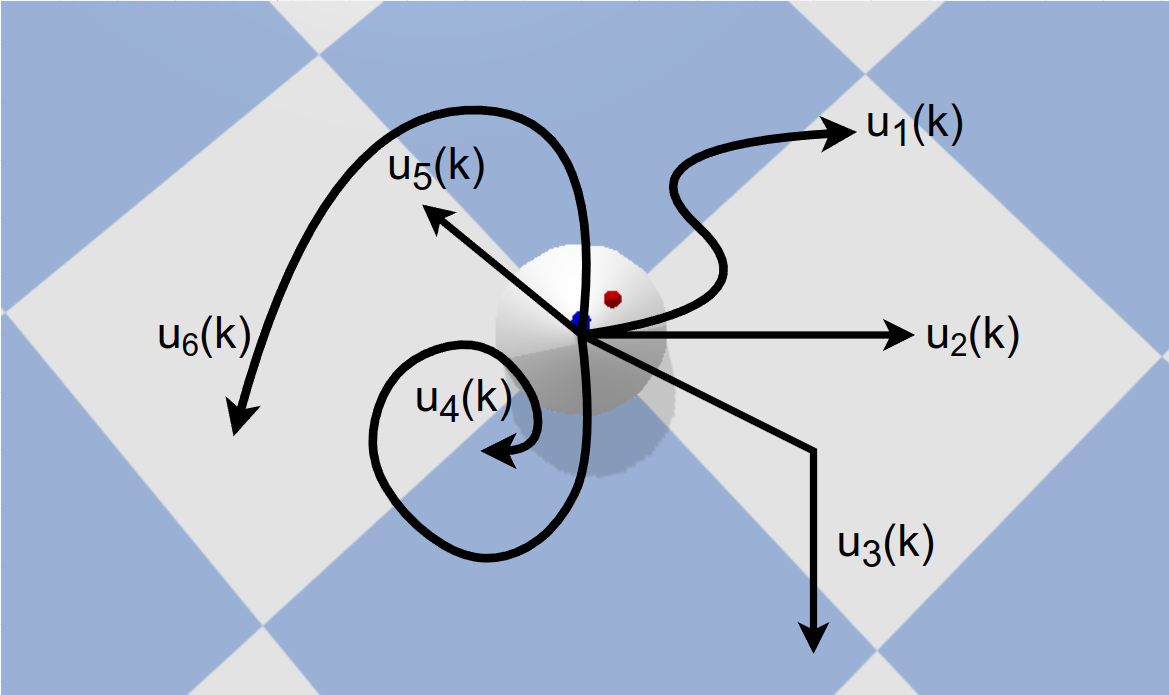
\includegraphics[width=0.5\textwidth]{figures/required_background/collect_io_data_robot}
  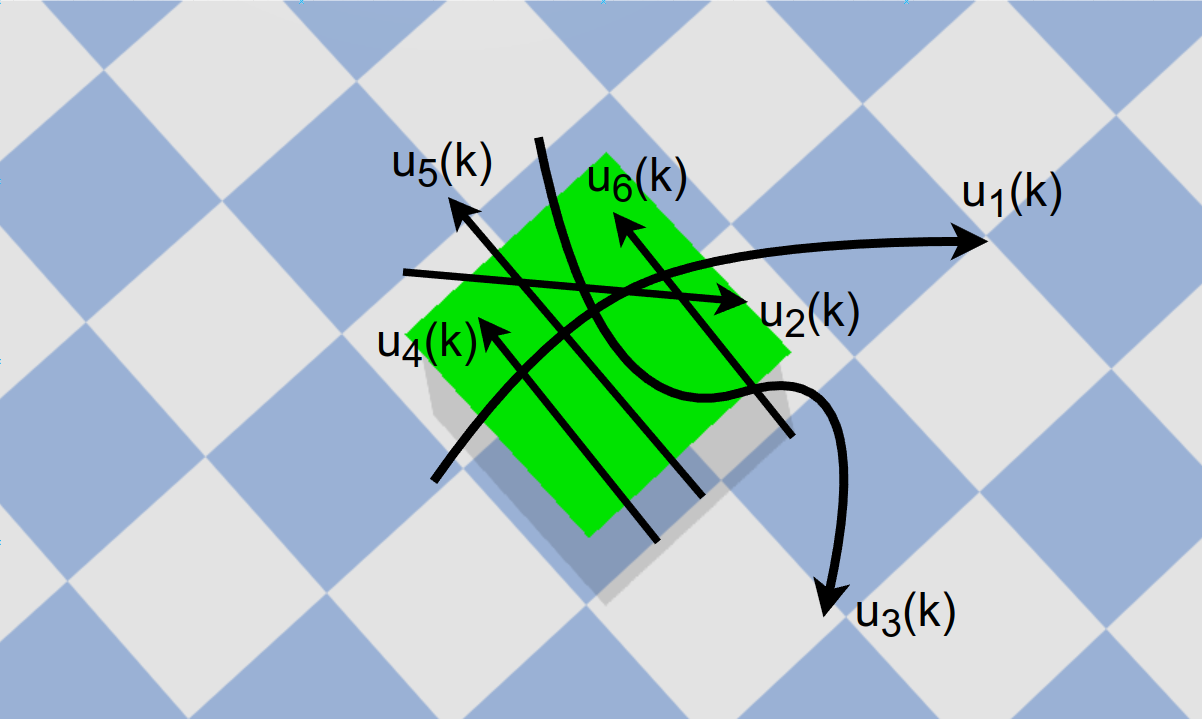
\includegraphics[width=0.5\textwidth]{figures/required_background/collect_io_data_object}
\end{center}
\end{frame}

\begin{frame}[fragile]{Required Background: System identification} % some commands, e.g. \verb require [fragile]
  \todo{gif that shows going toward pushing pose, then push}
\end{frame}

\begin{frame}[fragile]{Required Background: System identification} % some commands, e.g. \verb require [fragile]
  \[
x_{\mathit{lti-drive-model}}(k+1)=
\begin{bmatrix}
x_\mathit{robot}(k+1)\\
y_\mathit{robot}(k+1)
\end{bmatrix}
=
\begin{bmatrix}
x_{\mathit{robot}}(k) + DT u_{x}(k)\\
y_{\mathit{robot}}(k) + DT u_{y}(k)
\end{bmatrix}
\]

\[
x_{\mathit{lti-push-model}}(k+1)=
\begin{bmatrix}
x_{\mathit{robot}}(k+1)\\
y_{\mathit{robot}}(k+1)\\
x_{\mathit{obj}}(k+1)\\
y_{\mathit{obj}}(k+1)
\end{bmatrix}
=
\begin{bmatrix}
x_{\mathit{robot}}(k+1) + DT u_{x}(k)\\
y_{\mathit{robot}}(k+1) + DT u_{y}(k)\\
x_{\mathit{obj}}(k+1) + \frac{1}{2} DT u_{x}(k)\\
y_{\mathit{obj}}(k+1) + \frac{1}{2} DT u_{y}(k)
\end{bmatrix}
\]
\end{frame}

\begin{frame}[fragile]{Required Background: Control Methods} % some commands, e.g. \verb require [fragile]
  Both MPC and MPPI use a system model and an objective function. The main difference lies in 
  MPC uses a mathematical solver to obtain the best input, whilst MPPI samples random rollouts into the 
  future to then take the weighted average the results into the lowest cost function

  \begin{center}
  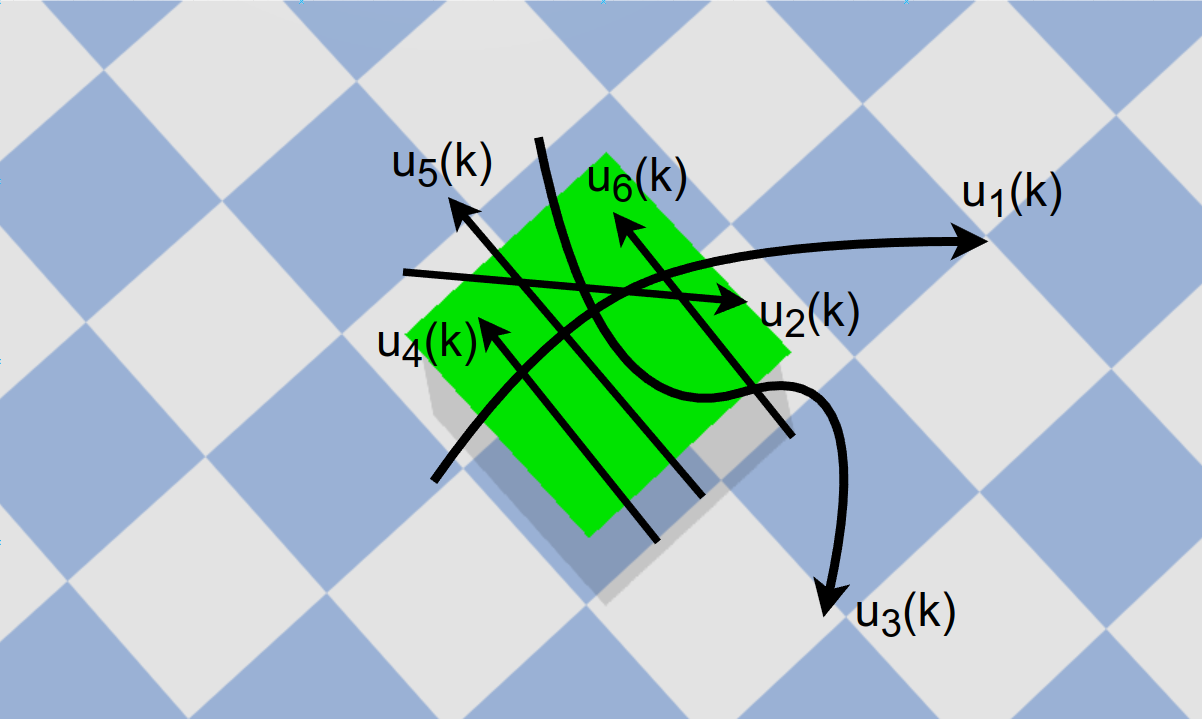
\includegraphics[width=0.5\textwidth]{figures/required_background/collect_io_data_object}
  \end{center}
\end{frame}

\begin{frame}[fragile]{Required Background: Planning a Path} % some commands, e.g. \verb require [fragile]
  \todo{image that has start and target for the robot in an interesting environment}
\end{frame}

\begin{frame}[fragile]{Required Background: Path Estimation} % some commands, e.g. \verb require [fragile]
\begin{block}{}
\begin{enumerate}
  \item Path Estimation\\\pause
  \item Path Planning\\
\end{enumerate}
\end{block}
\end{frame}


\begin{frame}[fragile]{Required Background: Path Estimation} % some commands, e.g. \verb require [fragile]
  \todo{with the image above, that interesting environment, create an occupancy grid}
\end{frame}

\begin{frame}[fragile]{Required Background: Path Estimation} % some commands, e.g. \verb require [fragile]


\begin{center}
\begin{tikzpicture}[scale=0.75, every node/.style={scale=0.75}]
    % Nodes
    \node [decision, text width=8em, line width=1pt] (first) { Can the path estimator find a path between start- and target configuration? };

    \node [block, below left=1cm and 1cm of first, minimum width=13em, text width=12em, line width=1pt] (path_exists) { A path does exist, however,it can still be unfeasible due to constraints other than the geometric constraints };
    \node [block, below right=1cm and 1cm of first, minimum width=13em, text width=12em, line width=1pt] (path_does_not_exists) { A path could not be found, however, due to the \textit{finite} discretization a path could exist and could not be found};

    \draw[>=stealth, ->, line width=1.0pt] (first.west) [out=180, in=90] to node[xshift=-0.3cm, above] {\large yes} (path_exists.north);
    \draw[>=stealth, ->, line width=1.0pt] (first.east) [out=0, in=90] to node[xshift=0.3cm, above] {\large no} (path_does_not_exists.north);
\end{tikzpicture}
\end{center}
\end{frame}

\begin{frame}[fragile]{Required Background: Planning} % some commands, e.g. \verb require [fragile]
  recap for RRT*

\end{frame}


\begin{frame}[fragile]{Required Background: Planning} % some commands, e.g. \verb require [fragile]
  recap for RRT*
  image of environment
  and make a video please
\end{frame}

